% Chapter 4

\chapter{A CUDA accelerated HMMER3 protein sequence search tool} % Main chapter title

\label{CUDAHMMER3} % For referencing the chapter elsewhere, use \ref{Chapter1} 

\lhead{Chapter \ref{CUDAHMMER3}. \emph{A CUDA accelerated HMMER3 protein sequence search tool}} % This is for the header on each page - perhaps a shortened title

%----------------------------------------------------------------------------------------

\section{Requirements and design decisions}

The following are the requirements for a CUDA accelerated HMMER3 protein sequence search tool:

\begin{itemize}
\item A HMMER3 protein sequence search tool, named cudaHmmsearch, will be implemented to run on CUDA-enabled GPU and several optimization will be taken to accelerate the computation. The cudaHmmsearch will be tested and compared with other CPU and GPU implementations.
\item The cudaHmmsearch will be based on HMMER3 algorithm so that the result will be same as hmmsearch of HMMER3.
\item The cudaHmmsearch will be completely usable under various GPU devices and sequence database size. This means that cudaHmmsearch is not just for research purpose or just a proof of concept.
\end{itemize}

\subsubsection*{Implementation toolkit and language}

NVIDIA CUDA \citep{CUDAzone} was chosen as the toolkit to be used in the implementation phase. Since its introduction in 2006, CUDA has been widely deployed through thousands of applications and published research papers, and supported by an installed base of over 500 million CUDA-enabled GPUs in notebooks, workstations, compute clusters and supercomputers \citep{CUDAwhat}. As of writing, CUDA is the most mature and popular GPU programming toolkit. 

HMMER3 is implemented in C programming language. CUDA provides a comprehensive development environment for C and C++ developers. However, some advanced features of CUDA, such as texture, are only supported in C++ template programming. So C++ has to be used, and some compatible problems when compiling and programming between C and C++ have also to be dealt with accordingly.

\subsubsection*{Implementation methods}
\label{impl}

The following two approaches have been explored for parallelizing the protein sequence database search using CUDA. A target sequence in the database is processed as one task.

\begin{itemize}
 \item \textbf{Task-based parallelism} Each task is assigned to exactly one thread, and \emph{dimBlock} tasks are performed in parallel by different threads in a thread block.
 \item \textbf{Data-based parallelism} Each task is assigned to one thread block and all \emph{dimBlock} threads in the thread block cooperate to perform the task in parallel.
\end{itemize}

Task-based parallelism has some advantages over data-based parallelism. On one side, it removes the need for inter-thread communications or, even worse, inter-multiprocessor communications. As described before, the thread or processing elements of one CUDA multiprocessor can communicate by using shared memory, while slow global memory must be used to transfer data between multiprocessors. At the same time, data-based also needs to take time on synchronizing and cooperating among threads. On the other side, to task-based, performing one sequence on each thread results in a kernel where each processing element is doing the exact same thing independently. This also simplifies implementation and testing. Although task-based parallelism needs more device memory than data-based, it can achieve better performance \citep{SW++}. Thus, the approach of task-based parallelism is taken and more efforts are put on optimizing CUDA kernel execution.

Since data-based parallelism occupies significantly less device memory, \citep{SW++} uses it to support longest query/subject sequences. However, different strategy here is applied to work around this problem and is discussed in details in subsection\ref{workload} on workload distribution.

%----------------------------------------------------------------------------------------

\section{A straightforward implementation}

This section describes a straightforward, mostly un-optimized implementation of the protein database search tool. First, a simple serial CPU implementation of hmmsearch is presented, with no GPU specific traits. Next, the MSV filter is ported to the GPU. This implementation is then optimized in the next section.

\subsection{CPU serial version of hmmsearch}

The CPU serial version of hmmsearch in HMMER3 is shown in Figure\ref{fig:hmmsearch}. The MSV and Viterbi algorithms described in subsection \ref{ViterbiSub} and \ref{MSVsub} are implemented in the so-called “acceleration pipeline” at the core of the HMMER3 software package \citep{HMMER3}. One call to the acceleration pipeline is executed for the comparison of each query model and target sequence.

\begin{figure}[!htb]
 \centering
 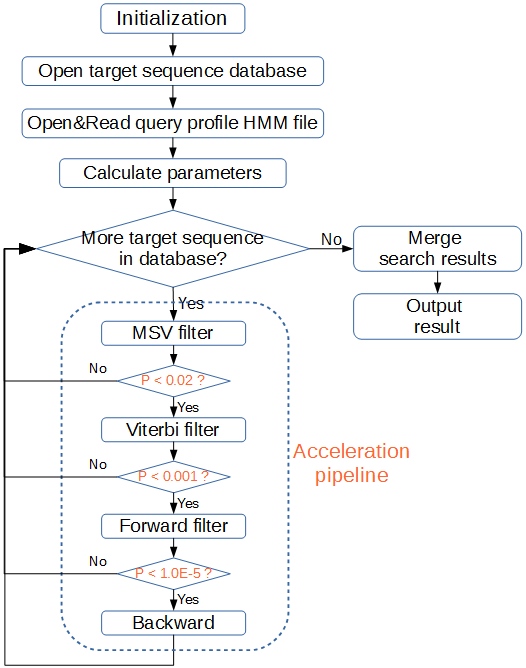
\includegraphics[totalheight=0.5\textheight]{Figures/hmmsearch.png}
 \caption{\fontfamily{pag}\selectfont The CPU serial version of hmmsearch}
 \label{fig:hmmsearch}
\end{figure}

\label{hmmsearch}
After each filter step, the pipeline either accepts or rejects the entire comparison, based on the P-value of the score calculated in each filter. For example, as can be seen in Figure\ref{fig:hmmsearch}, by default a target sequence can pass the MSV filter if its comparison gets a P-value of less than 0.02, which means the top-scoring 2\% of target sequences are expected to pass the filter. So, much fewer target sequence can pass one filter and need further computing. By this way, the comparison is accelerated. Thus, the first MSV filter is typically the run time bottleneck for hmmsearch. Therefore, the key to parallelizing hmmsearch tool is to offload the MSV filter function to multiple computing elements on GPU, while ensuring that the code shown in Figure\ref{MSV-SIMD} is as efficient as possible.

\subsection{GPU implementation of MSV filter}

A basic flow of the GPU implementation for MSV filter is shown in Figure\ref{fig:gpuMSV}. As can be seen, the code must be split up into two parts, with the left \emph{host} part running on CPU and the right \emph{device} part running on GPU. Some redundancy as data needed by GPU to compute will be copied around the memories in host and device.

\begin{figure}[!htb]
 \centering
 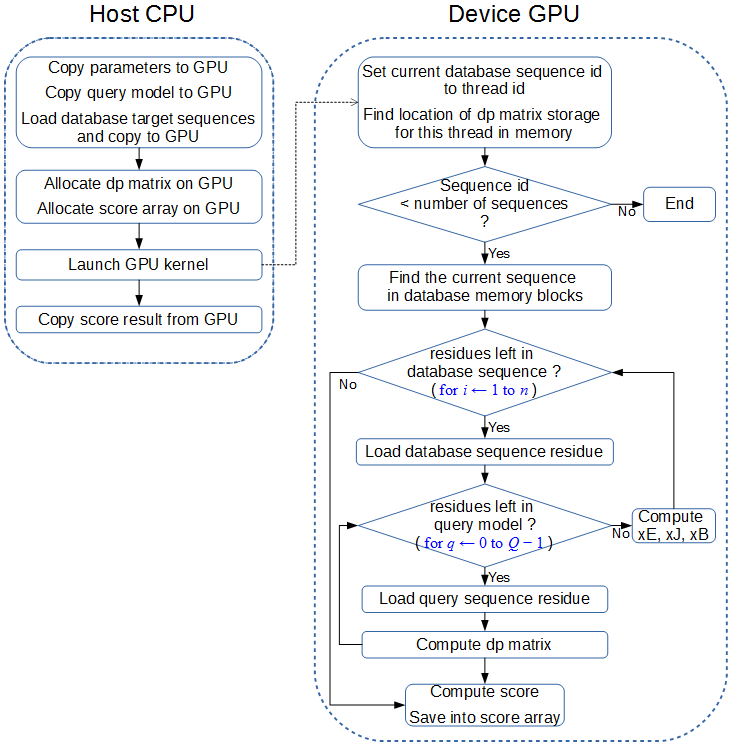
\includegraphics[totalheight=0.6\textheight]{Figures/gpuMSV.png}
 \caption{\fontfamily{pag}\selectfont The GPU porting of MSV filter}
 \label{fig:gpuMSV}
\end{figure}

The CPU code mainly concerns about allocating data structures on GPU, loading data, copying them to GPU, launching the GPU kernel and copying back the result for further steps.

The GPU kernel code is corresponding to the MSV filter Algorithm \ref{MSV-SIMD}. and Some more explanation are worth for it. First, the thread's current database sequence is set to the thread id. By this way each thread begins processing a different neighbouring sequence. This thread id is a unique numeric identifier for each thread and the id numbers of threads in a warp are consecutive. Next, the location where each thread can store and compute its dp matrix is determined in the global memory. This is calculated also using the thread id for each thread. When processing the sequence, successive threads access the successive addresses in the global memory for the sequence data and dp matrix, i.e. using a coalesced access pattern. Execution on GPU kernel is halted when each thread finishes its sequences.


%----------------------------------------------------------------------------------------

\section{Optimizing the implementation}

Although a fully functioning GPU MSV filter has been presented, its simple implementation is quite slow: more than 227 seconds to search a test database with 540,958 query sequences.

This section discusses the optimization steps taken to eventually reach a benchmark database search time of 1.55 seconds: an almost 147 times speedup.

\subsection{Global Memory Accesses}
\label{global}

The global memory is used to store most of data on GPU. A primary in the optimization is to improve the efficiency of accessing global memory as much as possible. One way of course is to reduce the frequency of access. Another way is coalescing access.

\subsubsection*{Access frequency}

The elements of the \emph{dp} matrix and the query profile 2D matrix are 8-bit value.  The \emph{uint4} and \emph{ulong2} (see the code below) are 128-bit CUDA built-in vector types. So the access frequency would be decreased 16 times by using \emph{uint4} or \emph{ulong2} to fetch the 8-bit value residing in global memory, compared with using 8-bit \emph{char} type.

\begin{quote}
\fontfamily{phv}\fontseries{m}\selectfont
struct \_\_device\_builtin\_\_ uint4\\
\{\\
   unsigned int x, y, z, w;\\
\}\\
struct \_\_device\_builtin\_\_ ulong2\\
\{\\
    unsigned long int x, y;\\
\};\\
\end{quote}
% \newcommand\codeHighlight[1]{\textcolor[rgb]{0,0,1}{\textbf{#1}}}
% \begin{Verbatim}[commandchars=\\\{\}]
% \codeHighlight{struct}  __device_builtin__ uint4
% \{
%     unsigned int x, y, z, w;
% \}
% \codeHighlight{struct} __device_builtin__ ulong2
% \{
%     unsigned long int x, y;
% \};
% \end{Verbatim}

This approach resulted in increased register pressure and gained a huge speed boost of almost 8 times in total.

\subsubsection*{coalescing access}

Coalescing access is the single most important performance consideration in programming for CUDA-enabled GPU architectures. Coalescing is a technique applied to combine non-contiguous and small reads/writes of global memory, into the single and more efficient contiguous and large memory reads. A prerequisite for coalescing is that the words accessed by all threads in a warp must lie in the same segment. As can be seen in Figure\ref{fig:coalescing}, the memory spaces referred to by the same variable names (not referring to same addresses) for all threads in a warp have to be allocated in the form of an array to keep them contiguous in address.

\begin{figure}[!htb]
	\centering
	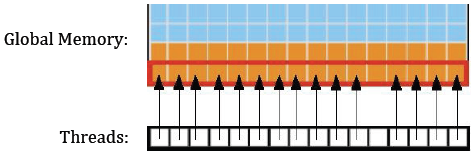
\includegraphics[totalheight=0.115\textheight]{Figures/coalesce.png}
	\caption{\fontfamily{pag}\selectfont Coalescing Global Memory Accesses\citep{Waters}.}
	\label{fig:coalescing}
\end{figure}

For coalescing access, the target sequences are arranged in an array like an upside-down bookcase shown in Figure\ref{fig:dbalign}, where all residues of a sequence are restricted to be stored in the same column from top to bottom. And all sequences are arranged in decreasing length order from left to right in the array, which is explained in section x. 

\begin{figure}[!htb]
	\centering
	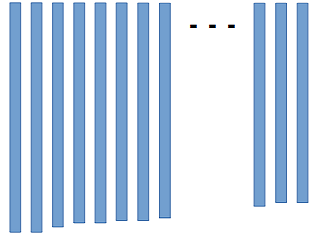
\includegraphics[totalheight=0.2\textheight]{Figures/dbalign.png}
	\caption{\fontfamily{pag}\selectfont Alignment of target sequences.}
	\label{fig:dbalign}
\end{figure}

Figure\ref{fig:dp} presents the similar global memory allocation pattern of \emph{dp} matrix for \emph{M} processing target sequences. Each thread processes independent \emph{dp} array with the same length \emph{Q}. A memory slot is allocated to a thread and is indexed top-to-bottom, and the access to \emph{dp} arrays is coalesced by using the same index for all threads in a warp.

\begin{figure}[!htb]
	\centering
	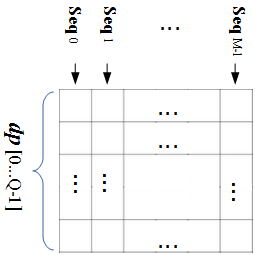
\includegraphics[totalheight=0.2\textheight]{Figures/dp.png}
	\caption{\fontfamily{pag}\selectfont The dp matrix in global memory.}
	\label{fig:dp}
\end{figure}

An alignment requirement is needed to fulfill for fully coalescing, which means any access to data residing in global memory is compiled to a single global memory instruction. The alignment requirement is automatically fulfilled for the built-in types like \emph{uint4} \citep{CUDA-C}.

The move to vertical alignment of \emph{dp} matrix resulted in an improvement of about 44\%.

\subsubsection*{Note on coding global memory coalescing access}
At the beginning, the traditional C/C++ memory block copy function \emph{memcpy}() was used, since uint4 is 16-bytes block. \emph{dp} is the pointer to the address of global memory. \emph{mpv} and \emph{sv} are \emph{uint4} data residing in register memory.

\begin{quote}
\fontfamily{phv}\fontseries{m}\selectfont
 memcpy(\&mpv, dp, sizeof(uint4));\\
 memcpy(dp, \&sv, sizeof(uint4));
\end{quote}

% \begin{lstlisting}[frame=none]
% memcpy(&mpv, dp, sizeof(uint4));
% memcpy(dp,  &sv, sizeof(uint4));
% \end{lstlisting}

However, in practice of CUDA kernel execution, the above \emph{memcpy} involves 16 (sizeof(uint4)) reads and writes respectively. This does not fully coalesce access global memory. Switching to the following direct assignment resulted in 81\% improvement.

\begin{quote}
\fontfamily{phv}\fontseries{m}\selectfont
 mpv = *(dp);\\
 *(dp) = sv;
\end{quote}

\subsection{texture memory}
\label{tex}

The read-only texture memory space is a cached window into global memory that offers much lower latency and does not require coalescing for best performance. Therefore, a texture fetch costs one device memory read only on a cache miss; otherwise, it just costs one read from the texture cache. The texture cache is optimized for 2D spatial locality, so threads of the same warp that read texture addresses that are close together will achieve best performance \citep{CUDA-C}.

Texture memory is well suited to random access. CUDA has optimized the operation fetching four values (RGB colors and alpha component, a typical graphics usage) at a time in texture memory. And this mechanism is also applied to fetch four values from the query profile 2D matrix with the \emph{uint4} built-in type. Since the data of target sequences is read-only, it can also use texture for better performance.

Switching to texture memory for the query profile texOMrbv resulted in about 22\% performance improvement.

\subsubsection*{Restrictions using texture memory}

Texture memory come from the GPU graphics and therefore are less flexible than the CUDA standard types. It must be declared at compile time as a fixed type, \emph{uint4} for the query profile in our case:

\begin{quote}
\fontfamily{phv}\fontseries{mc}\selectfont
 texture$<$uint4, cudaTextureType2D, cudaReadModeElementType$>$ \emph{texOMrbv};
\end{quote}

How the values are interpreted is specified at run time. Texture memory is read-only to CUDA kernel and must be explicitly accessed via a special texture API (e.g. tex2D(), tex1Dfetch(), etc) and arrays bound to textures.

\begin{quote}
\fontfamily{phv}\fontseries{m}\selectfont
 uint4 rsc4 = tex2D(texOMrbv, x, y);
\end{quote}

However, on the CUDA next-generation architecture Kepler, the texture cache gets a special compute path, removing the complexity associated with programming it \citep{Kepler}.

\subsection{Virtualized SIMD vector programming model}

Inspired by the fact that CUDA has optimized the operation fetching a four component RGBA colour in texture memory, the target sequences is re-organized using a packed data format, where four consecutive residues of each sequence are packed together and represented using the \emph{uchar4} vector data type, instead of the \emph{char} scalar data type, as can be seen in Figure\ref{fig:simdvector}(\textit{a}). In this way, four residues are loaded using only one texture fetch, thus significantly improving texture memory throughput. 

\begin{figure}[!htb]
	\centering
	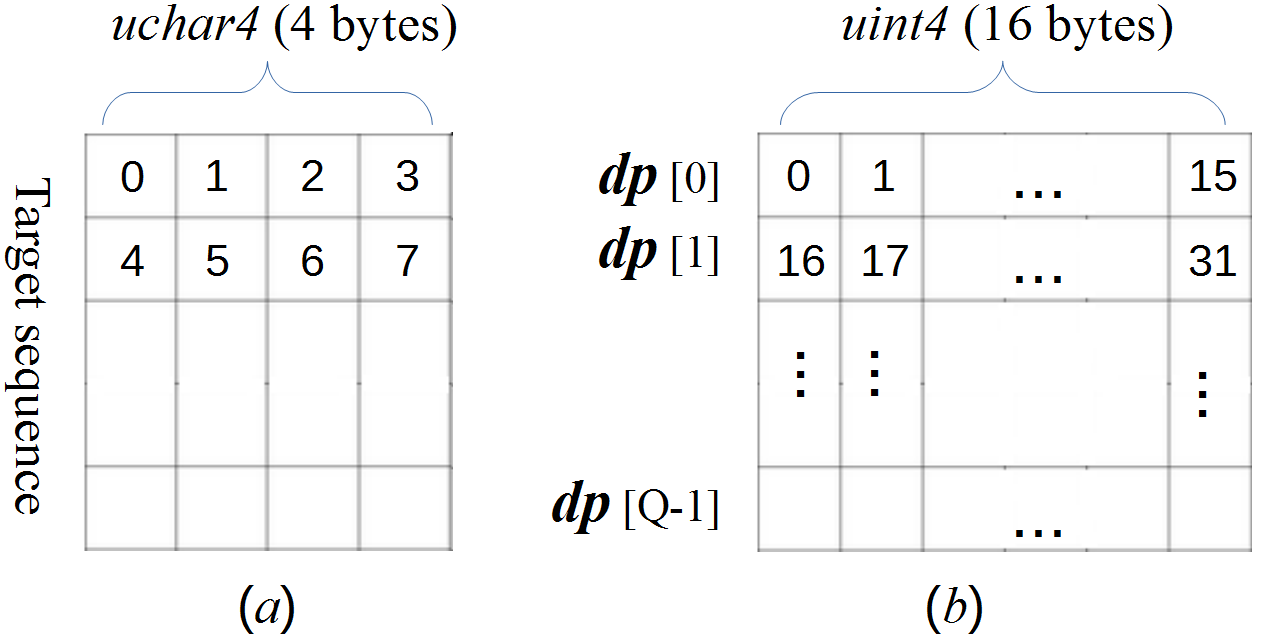
\includegraphics[totalheight=0.2\textheight]{Figures/simdvector.png}
	\caption{\fontfamily{pag}\selectfont SIMD vector alignment of data: (\textit{a}) target sequence; (\textit{b}) dp array.}
	\label{fig:simdvector}
\end{figure}

Similarly, the dp array and the query profile also use the virtualized SIMD vector allocation pattern, as can be seen in Figure\ref{fig:simdvector}(\textit{b}).

\subsection{SIMD Video Instructions}
\label{video}

Like Interl SSE2 described in subsection\ref{SSE2}, CUDA also provides the scalar SIMD (Single Instruction, Multiple Data) video instructions. These are available on devices of compute capability 3.0. The SIMD video instructions enable efficient operations on pairs of 16-bit values and quads of 8-bit values needed for video processing.

The SIMD video instructions can be included in CUDA programs by way of the assembler, \emph{asm}(), statement.

The basic syntax of an \emph{asm}() statement is:

\begin{quote}
\fontfamily{phv}\fontseries{m}\selectfont
 asm(``template-string" : ``constraint''(output) : ``constraint"(input));
% \slshape A narrow slanted f\'ee.\\
\end{quote}

The following three instructions are used in the implementation. Every instruction operates on quads of 8-bit signed values. The source operands(“op1” and “op2”) and destination operand(“rv”) are all unsigned 32-bit registers(“u32”), which is different from 128-bit in SSE2. For additions and subtractions, saturation instructions(“sat”) have been used to clamp the values to their appropriate unsigned ranges.

\begin{quote}
\fontfamily{phv}\fontseries{mc}\selectfont
 \textsl{/* rv[z] = op1[z] + op2[z] (z = 0,1,2,3) */}\\
 asm(``vadd4.u32.u32.u32.sat \%0, \%1, \%2, \%3;" : ``=r"(rv) : ``r"(op1), ``r"(op2), ``r"(0));\\
 \textsl{/* rv = op1 + op2 */}\\
 asm(``vsub4.u32.u32.u32.sat \%0, \%1, \%2, \%3;" : ``=r"(rv) : ``r"(op1), ``r"(op2), ``r"(0));\\
 \textsl{/* rv = max(op1,op2) */}\\
 asm(``vmax4.u32.u32.u32 \%0, \%1, \%2, \%3;" : ``=r"(rv) : ``r"(op1), ``r"(op2), ``r"(0));
% \slshape A narrow slanted f\'ee.\\
\end{quote}

Switching to the SIMD video instructions also achieved a large speedup of nearly 2 times.

\subsection{Pinned (non-pageable) Memory}
\label{pin}

It is necessary to transfer data to the GPU over the PCI-E data bus. Compared to access to CPU host memory, this bus is very slow. Pinned memory is memory that cannot be paged (swapped) out to disk by the virtual memory management of the OS. In fact, PCI-E transfer can only be done using pinned memory, and if the application does not allocate pinned memory, the CUDA driver does this in the background for us. Unfortunately, this results in a needless copy operation from the regular (paged) memory to or from pinned memory. We can of course eliminate this by allocating pinned memory ourselves.

In the application, we simply replace \emph{malloc/free} when allocating/freeing memory in the host application with \emph{cudaHostAlloc/cudaFreeHost}.

\begin{quote}
\fontfamily{phv}\fontseries{m}\selectfont
 cudaHostAlloc (void** host\_pointer, size\_t size, unsigned int flags)
\end{quote}

\subsection{Asynchronous memory copy and Streams}
\label{asyn}

\subsubsection*{Asynchronous memory copy}
By default, any memory copy involving host memory is synchronous: the function does not return until after the operation has been completed. This is because the hardware cannot directly access host memory unless it has been page-locked or pinned and mapped for the GPU. An asynchronous memory copy for pageable memory could be implemented by spawning another CPU thread, but so far, CUDA has chosen to avoid that additional complexity.

Even when operating on pinned memory, such as memory allocated with \emph{cudaMallocHost}(), synchronous memory copy must wait until the operation is finished because the application may rely on that behavior. When pinned memory is specified to a synchronous memory copy routine, the driver does take advantage by having the hardware use DMA, which is generally faster \citep{CUDAHand}.

When possible, synchronous memory copy should be avoided for performance reasons. Keeping all operations asynchronous improves performance by enabling the CPU and GPU to run concurrently. Asynchronous memory copy functions have the suffix \emph{Async}(). For example, the CUDA runtime function for asynchronous host to device memory copy is \emph{cudaMemcpyAsync}().

It works well only where either the input or output of the GPU workload is small in comparison to one another and the total transfer time is less than the kernel execution time. By this means we have the opportunity to hide the input transfer time and only suffer the output transfer time.

\subsubsection*{Multiple streams}
A CUDA stream represents a queue of GPU operations that get executed in a specific order. We can add operations such as kernel launches, memory copies, and event starts and stops into a stream. The order in which operations are added to the stream specifies the order in which they will be executed. CUDA streams enable CPU/GPU and memory copy/kernel processing concurrency. For GPUs that have one or more copy engines, host $\longleftrightarrow$ device memory copy can be performed while the SMs are processing kernels. Within a given stream, operations are performed in sequential order, but operations in different streams may be performed in parallel \citep{CUDAintro}.

To take advantage of CPU/GPU concurrency as depicted in Figure\ref{fig:cpu_gpu}, when performing memory copies as well as kernel launches, asynchronous memory copy must be used. And Mapped pinned memory can be used to overlap PCI Express transfers and kernel processing.

\begin{figure}[!htb]
	\centering
	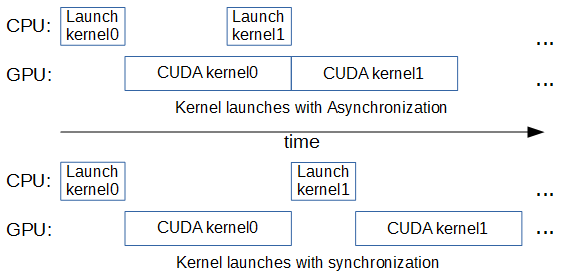
\includegraphics[totalheight=0.3\textwidth]{Figures/cpu_gpu.png}
	\caption{\fontfamily{pag}\selectfont CPU/GPU concurrency.}
	\label{fig:cpu_gpu}
\end{figure}

CUDA compute capabilities above 2.0 are capable of concurrently running multiple kernels, provided they are launched in different streams and have block sizes that are small enough so a single kernel will not fill the whole GPU.

By using multiple streams, we broke the kernel computation into chunks and overlap the memory copies with kernel execution. The new improved implementation might have the execution timeline as shown in Figure\ref{fig:streams} in which empty boxes represent time when one stream is waiting to execute an operation that it cannot overlap with the other stream's operation.

\begin{figure}[!htb]
	\centering
	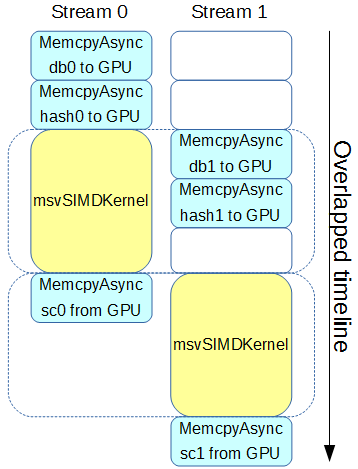
\includegraphics[totalheight=0.32\textheight]{Figures/streams.png}
	\caption{\fontfamily{pag}\selectfont Timeline of intended application execution using two independent streams.}
	\label{fig:streams}
\end{figure}
% \begin{lstlisting}[language=C++, caption={Combined asynchronous memory copy and multiple streams}, captionpos=t]
% // enqueue copies of dbQuad in stream0 and stream1
% cudaMemcpyAsync(cudaPtr.dbQuad0, hostPtr.dbQuad0,
% 		num0 * sizeof(uint),
% 		cudaMemcpyHostToDevice,
% 		stream[0]);
% cudaMemcpyAsync(cudaPtr.dbQuad1, hostPtr.dbQuad1,
% 		num2 * sizeof(uint),
% 		cudaMemcpyHostToDevice,
% 		stream[1]);
% 
% // enqueue copies of hashQuad in stream0 and stream1
% cudaMemcpyAsync(cudaPtr.hashQuad0, hostPtr.hashQuad0, num0 * sizeof(uint), cudaMemcpyHostToDevice, stream[0]);
% cudaMemcpyAsync(cudaPtr.hashQuad1, hostPtr.hashQuad1, num1 * sizeof(uint), cudaMemcpyHostToDevice, stream[1]);
% 
% // enqueue kernels in stream0 and stream1
% msvSIMDKernel0<<<numBlocks, KERNEL_BLOCKSIZE, 0, stream[0]>>>();
% msvSIMDKernel0<<<numBlocks, KERNEL_BLOCKSIZE, 0, stream[1]>>>();
% 
% // enqueue copies of result from device to locked memory
% cudaMemcpyAsync(hostSC0, cudaSC0, num0 * sizeof(float), cudaMemcpyDeviceToHost, stream[0]);
% cudaMemcpyAsync(hostSC1, cudaSC1, num1 * sizeof(float), cudaMemcpyDeviceToHost, stream[1]);
% \end{lstlisting}

Running the improved program using pinned memory, asynchronous memory copy and two streams reveals the time drops from 16.45s to just 9.46s, a quite significant drop of over 73.8\% in execution time.

\subsection{Sorting database}
\label{dbsort}
As described in Section\ref{MSVsub}, MSV filter function is sensitive to the length of a target sequence, which determines the execution times of main \emph{for} loop in Algorithm\ref{MSV-SIMD}. 

Target sequence database could contain many sequences with different lengths.  The 24GB NCBI NR database consists of over 38 million sequences with sequence lengths varying from 6 $\sim$ 37,000+ amino acids \citep{NCBI}.

This brings a problem for parallel processing of threads on GPU: one thread could be processing a sequence of several thousands of residues while another might be working on a sequence of just a few. As a result, the thread that finishes first might be idle while the long sequence is being handled. Furthermore, unless care is taken when assigning sequences to threads, this effect might be compounded by the heavily unbalanced workload among threads.

In order to achieve high efficiency for task-based parallelism, the run time of all threads in a thread block should be roughly identical. Therefore the database is converted with sequences being sorted by length. Thus, for two adjacent threads in a thread warp, the difference value between the lengths of the associated sequences is minimized, thereby balancing a similar workload over threads in a warp.

\subsubsection*{Block reading}
Many research implementation were not concerned with practical matters. They just loaded the whole database data into memories of CPU host and GPU device. Large database, like NCBI NR database, is more than 24GB in size and is still increasing, being too large to load into memories of most machines.

Given GPU global memory is much less than CPU host, we use the size of GPU global memory as the basis to decide the size of sequence block while reading the database.

\subsubsection*{Descending order}
The memory pools for database sequences both in CPU host and GPU device are dynamically allocated at run time. The pools may be required to reallocated due to more space needed for the current data block than the last one. If the pool allocated at the first time is the largest one during execution, then the overhead of reallocation will be saved. Hence, the descending order is used for sorting the database.

\subsubsection*{Performance improved}
The CUDA profiling tool nvprof \citep{Profiler} was used to understand and optimize the performance of the MSV GPU application cudaHmmsearch. The nvprof command was used as follows:

\begin{quote}
\fontfamily{phv}\fontseries{m}\selectfont
 \# nvprof  ./cudaHmmsearch globins4.hmm uniprot\_sprot.fasta
\end{quote}

The table\ref{tab.nvprof1} and \ref{tab.nvprof2} list the profiling results of before and after the target database was sorted.

\begin{table}[H]
\centering
\begin{tabular}{|c|c|c|c|c|c|c|}\hline
\shortstack{\textbf{Time(\%)}} & \shortstack{\textbf{Time}} & \shortstack{\textbf{Calls}} & \shortstack{\textbf{Avg}} & \shortstack{\textbf{Min}} & \shortstack{\textbf{Max}} & \shortstack{\textbf{Name}} \\\hline
91.61\% & 4.27108s & 134 & 31.874ms & 5.9307ms & 137.67ms & msvSIMDKernel\\\hline
8.37\% & 390.01ms & 271 & 1.4391ms & 704ns& 23.027ms& [CUDA memcpy HtoD]\\\hline
0.01\% & 556.21us & 134 & 4.1500us & 1.7280us & 5.9840us& [CUDA memcpy DtoH]\\\hline
0.01\% & 491.23us & 134 & 3.6650us & 3.4880us& 4.0640us& [CUDA memset]\\\hline
\end{tabular}
\caption{\fontfamily{pag}\selectfont\textbf{Profiling result of before sorting database.} Each row is the statistics of profiling result for the function named in the `\textbf{Name}'. The statistics includes the percentage of running time, the running time, the number of called times, as well as the average, minimum, and maximum time.\label{tab.nvprof1}}
\end{table}

\begin{table}[H]
\centering
\begin{tabular}{|c|c|c|c|c|c|c|}\hline
\shortstack{\textbf{Time(\%)}} & \shortstack{\textbf{Time}} & \shortstack{\textbf{Calls}} & \shortstack{\textbf{Avg}} & \shortstack{\textbf{Min}} & \shortstack{\textbf{Max}} & \shortstack{\textbf{Name}} \\\hline
97.41\% & 2.07263s & 134 & 15.467ms & 29.056us & 194.91ms & msvSIMDKernel\\\hline
2.54\% & 54.115ms & 271 & 199.69us & 704ns& 23.013ms& [CUDA memcpy HtoD]\\\hline
0.03\% & 550.53us & 134 & 4.1080us & 1.6640us & 4.6720us& [CUDA memcpy DtoH]\\\hline
0.02\% & 474.90us & 134 & 3.5440us & 672ns& 4.0320us& [CUDA memset]\\\hline
\end{tabular}
\caption{\fontfamily{pag}\selectfont\textbf{Profiling result of after sorting database.} The meaning of each column is same as Table\ref{tab.nvprof1}\label{tab.nvprof2}}
\end{table}

From the result of profiling, we can see the performance has been increased, which is clearly shown in two ways:
\begin{enumerate}
 \item the ratio of the msvSIMDKernel run-time to the total increased from 91.61\% to 97.41\%;
 \item the  msvSIMDKernel run-time decreased from 4.27108s to 2.07263s and the time of the memory copy from Host to Device (CUDA memcpy HtoD) decreased from 390.01ms to 54.115ms.
\end{enumerate}

This approach has the advantage of being both effective and quite straightforward as a large 129\% performance improvement can be gained over the unsorted database without changing the GPU kernel in any way (see Table\ref{tab.opt} and Figure\ref{fig:imp}). For the 24GB NCBI NR database used in these experiments, only 6 minutes were taken for sorting. Further, the sorted database can still be usable for other applications, making the one-time cost of sorting it negligible.

\subsection{Distributing workload}
\label{workload}
After launching GPU kernel, CPU must wait for the GPU to finish before copying back the result. This is accomplished by calling \emph{cudaStreamSynchronize}( \emph{stream} ). We can get further improvement by distribute some work from GPU to CPU while CPU is waiting. In protein database, the sequences with the longest or the shortest length are very few. According to Swiss-Prot database statistics \citep{Swiss-Prot}, the percentage of sequences with length $>$ 2500 is only 0.2\%. Considering the length distribution of database sequences and based on the descending sorted database discussed in section\ref{dbsort}, we assigned the first part of data with longer lengths to CPU. By this way, we can save both the GPU global memory allocated for sequences and the overheads of memory transfer.

The compute power of CPU and GPU should be taken into consideration in order to balance the workload distribution between CPU and GPU. The distribution policy calculates a ratio \emph{R} of the number of database sequences assigned to GPU, which is calculated as

\begin{equation*}
   R = \frac{N_Gf_G}{N_Gf_G + f_C}
\end{equation*}

where $f_G$ and $f_C$ are the core frequencies of GPU and CPU, $N_G$ is the number of GPU Multiprocessors.

%----------------------------------------------------------------------------------------

\subsection{Miscellaneous consideration}
This sections discusses various small-scale optimization and explains some techniques not suited to the MSV implementation.

\subsection*{Data type for register memory}
\label{register}
In order to reduce the register pressure in CUDA kernel, we may consider using unsigned 8-bit char type (u8) instead of 32-bit int type (u32). Declaring the registers as u8 results in sections of code to shift and mask data. The extract data macros are deliberately written to mask off the bits that are not used, so this is entirely unnecessary. In fact, around four times the amount of code will be generated if using an u8 type instead of an u32 type.

Changing the u8 definition to an u32 definition benefits from eliminating huge numbers of instructions. It seems potentially wasting some register space. In practice, CUDA implements u8 registers as u32 registers, so this does not actually cost anything extra in terms of register space \citep{cook}.

\subsubsection*{Branch divergence}
\label{branch}

A warp executes one common instruction at a time, so full efficiency is realized when all 32 threads of a warp agree on their execution path. If threads of a warp diverge via a data-dependent conditional branch, the warp serially executes each branch path taken, disabling threads that are not on that path, and when all paths complete, the threads converge back to the same execution path. Branch divergence occurs only within a warp; different warps execute independently regardless of whether they are executing common or disjoint code paths. So the divergence results in some slowdown.

Since the implementation has changed u8 type in register memory to u32 type, the test for the overflow condition is not needed any more. This not only saves several instructions, but also avoids the issue of branch divergence.

\subsubsection*{Constant memory}
\label{constant}
Constant memory is as fast as reading from a register as long as all threads in a warp read the same 4-byte address. Constant memory does not support, or benefit from, coalescing, as this involves threads reading from different addresses. Thus, parameters used by all threads, such as $base$, $t_{jb}$, $t_{ec}$, are stored into constant memory.

\subsubsection*{Shared memory}
\label{shared}
In terms of speed, shared memory is perhaps 10x slower than register accesses but 10x faster than accesses to global memory. However, some disadvantages apply to shared memory.

\begin{itemize}
 \item Unlike the L1 cache, the shared memory has a per-block visibility, which would mean having to duplicate the data for every resident block on the SM.
 \item Data must be loaded from global to shared memory in GPU kernel and can not be uploaded to shared memory directly from the host memory.
 \item Shared memory is well suited to exchange data between CUDA threads within a block. As described in subsection\ref{impl}, task-based parallelism is applied without the need for inter-thread communications, which also saves the cost of synchronization \emph{\_\_syncthreads}() among threads.
\end{itemize}

Because of these disadvantages, the MSV implementation does not use shared memory.

\subsubsection*{Kernel launch configuration}
\label{launch}
Since the MSV implementation does not use shared memory explained above, the following dynamic kernel launch configuration is used to prefer larger L1 cache and smaller shared memory so as to further improve memory throughput.
\begin{quote}
\fontfamily{phv}\fontseries{m}\selectfont
 cudaFuncSetCacheConfig(msvSIMDKernel, cudaFuncCachePreferL1);
\end{quote}

%----------------------------------------------------------------------------------------

\section{Conclusion of optimization}
Summary of optimization steps taken

This section briefly reviews the all the optimization approaches discussed in this chapter thus far, and summarizes the steps to gain better performance for CUDA programming.

\subsection*{Six steps to better performance}
\begin{enumerate}
 \item Assessing the application\\
 In order to benefit from any modern processor architecture, including GPUs, the first steps are to assess the application to identify the hotspots [MSV filter in Section\ref{hmmsearch}], which type of parallelism [Task-based parallelism in Section\ref{impl}] is better suited to the application.
 \item Application Profiling\\
 NVIDIA® provides profiling tools to help execute the kernels in question under the watchful gaze [nvprof in Section\ref{dbsort}], which are publicly available as a separate download on the CUDA Zone website \citep{CUDAzone}.
 
% \begin{table}[H]
% \centering
% \begin{tabular}{|c|c|c|c|}\hline
% \shortstack{\textbf{Tools Name}} & \shortstack{\textbf{Command}} & \shortstack{\textbf{OS}} & \shortstack{\textbf{User interface}}\\\hline
% nvprof & nvprof & \shortstack{Linux, Mac OS X\\ and Windows} & command-line\\\hline
% Visual Profiler & nvvp & \shortstack{Linux, Mac OS X\\ and Windows} & graphical \\\hline
% Nsight™ Ecipse Edition & nsight & Linux and Mac OSX & graphical\\\hline
% \shortstack{NVIDIA® Nsight™ \\ Visual Studio Edition} & -\tablefootnote[12]{Integrated into Microsoft Visual Studio} & Windows & graphical\\\hline
% Parallel Nsight™ & - & Windows & graphical\\\hline
% \end{tabular}
% \caption{CUDA profiling tools\label{tab.prof}}
% \end{table}

\begin{table}[H]
\centering
\begin{tabular}{|c|c|c|c|}\hline
\shortstack{\textbf{Tools Name}} & \shortstack{\textbf{OS}} & \shortstack{\textbf{User interface}}\\\hline
nvprof & \shortstack{Linux, Mac OS X\\ and Windows} & command-line\\\hline
Visual Profiler & \shortstack{Linux, Mac OS X\\ and Windows} & graphical \\\hline
Nsight™ Ecipse Edition & Linux and Mac OSX & graphical\\\hline
\shortstack{NVIDIA® Nsight™ \\ Visual Studio Edition} & Windows & graphical\\\hline
Parallel Nsight™ & Windows & graphical\\\hline
\end{tabular}
\caption{\fontfamily{pag}\selectfont\textbf{CUDA profiling tools}\label{tab.prof}}
\end{table}

 \item Optimizing memory usage\\
 Optimizing memory usage starts with minimizing data transfers both in size [Data-base sorted in Section\ref{dbsort}, workload distribution in Section\ref{workload}] and time [Pinned Memory in Section\ref{pin}] between the host and the device [Asynchronous memory copy in Section\ref{asyn}]. Be careful with CUDA memory hierarchy: register memory [Section\ref{register}], local memory, shared memory [Section\ref{shared}], global memory, constant memory [Section\ref{constant}] and texture memory [Section\ref{tex}], and combine these memories to best suit the application [Kernel launch configuration in Section\ref{launch}]. Sometimes, the best optimization might even be to avoid any data transfer in the first place by simply recomputing the data whenever it is needed.\\
 The next step in optimizing memory usage is to organize memory accesses according to the optimal memory access patterns. This optimization is especially important for coalescing global memory accesses [Section\ref{global}].
 
 \item Optimizing instruction usage\\
 This suggests using SIMD Video Instructions [Section\ref{video}] and trading precision for speed when it does not affect the end result, such as using intrinsic instead of regular functions or single precision instead of double precision [HMMER3 in Section\ref{SSE2}]. Particular attention should be paid to control flow instructions [Branch divergence in Section\ref{branch}].
 
 \item Maximizing parallel execution
 
 The application should maximize parallel execution at a higher level by explicitly exposing concurrent execution on the device through streams [Section\ref{asyn}], as well as maximizing concurrent execution between the CPU host  [Database sorted in Section\ref{dbsort}] and the GPU device [Workload distribution in Section\ref{workload} and SIMD Video Instructions in Section\ref{video}].
 
 \item Considering the existing libraries
 
 Many existing GPU-optimized libraries \citep{CUDAlibs} such as cuBLAS \citep{cuBLAS}, MAGMA \citep{MAGMA}, ArrayFire \citep{ArrayFire}, or Thrust \citep{thrust}, are available to make the expression of parallel code as simple as possible.
 
\end{enumerate}


